%-----------------------------------------------------------------------------------------------
\chapter{Markers}\label{sect:marker}
%-----------------------------------------------------------------------------------------------

One of the goals of this project was to design a fiducial marker with advantageous properties for use in pose estimation.
In a typical scenario the marker may be seen from largely varying viewpoints.
Therefore it has to have some level of scale invariability.
If the observer is far from the marker, the smaller details may be lost due to the limited resolution of the camera.
If the same observer moves closer to the marker, it may fill the whole field of view and some features may even slip off the image.
This leads to another feature the marker needs: redundancy.
If the observer gets too close to the marker or some obstacle partially blocks the view, the localisation still needs to provide usable results.

The intended use of the markers is spatial localisation and pose estimation.
In other words: approximating the observers 3D coordinates ($x, y, z$) and orientation ($\phi, \theta, \psi$) with respect to the marker.
It is supposed that the observer uses a single camera system for navigation (e.g. smartphone or robotic application with limited resources).
This means the marker needs at least 6 degree of freedom.

To sum up the above discussed specifications, a suitable marker would have to:
\begin{itemize}
	\item have at least 6 DOF
	\item be (to some degree) scale invariant
	\item have redundancy
\end{itemize}

In the following sections will be a recommendation for a marker conforming for the listed specifications.
It is based on 3 connected line segments forming a quad with one missing side.
The whole marker is built from quads with different sides and angles.

%-----------------------------------------------------------------------------------------------
\section{Quad}
%-----------------------------------------------------------------------------------------------

A marker is put together from quads.
Figure \figref{exampleQuads} shows two examples.
One side of the quads is left out: they are put together from three joint line segments.
The middle segment, with two adjoining lines, will be referred to as the 'base' of the quad.
The outer segments are going to be called 'arms'.

\begin{figure}
	\begin{subfigure}{0.5\textwidth}
		\centering
		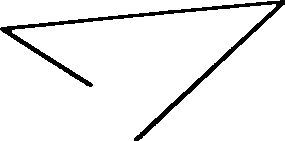
\includegraphics[width=0.75\textwidth]{figures/quad1.png}
	\end{subfigure}
	\begin{subfigure}{0.5\textwidth}
		\centering
		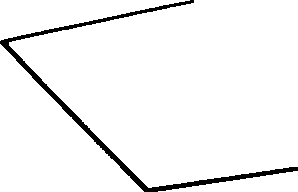
\includegraphics[width=0.75\textwidth]{figures/quad2.png}
	\end{subfigure}
	\caption{Example for different quads}
	\label{fig:exampleQuads}
\end{figure}

A quad has 6 degrees of freedom.
There are 3 independent distance parameters: the length of the base and the two arm segments.
There are also 3 unrelated angle parameters: the angles between each arm and the base, and the orientation of the quad.

\begin{figure}[ht]
	\centering
	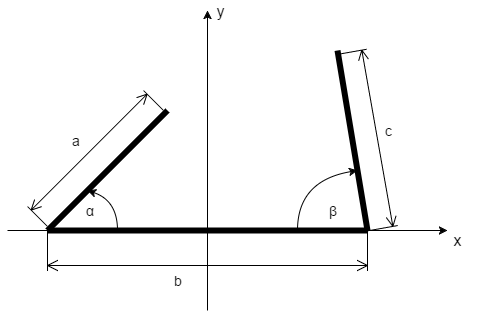
\includegraphics[width=0.75\textwidth]{figures/quad_params.png}
	\caption{Quad parameters}
	\label{fig:quadParams}
\end{figure}

Figure \figref{quadParams} shows the free parameters of a quad (the orientation is not shown on the image).
The following notation is used:
\begin{itemize}
	\item[a]: The length of one arm
	\item[b]: The length of the base
	\item[c]: The length of the other arm
	\item[$\alpha$]: The angle between one arm and the base
	\item[$\beta$]: The angle between the other arm and the base
	\item[$\gamma$]: The angle with which the whole quad is rotated
\end{itemize}
For the sake of simplicity, figure \figref{quadParams} does not show the rotation with $\gamma$.
The quad would be rotated around the origin of it's coordinate system.

The value of the length parameters are given in pixels, although they can be expressed in any unit of distance.
The angles can be given is degrees of radians (in the implementation degrees are used for easier human readability).

\begin{equation}
	a\in(0 , a_{max}]
	\label{eq:aRange}
\end{equation}
\begin{equation}
	b\in(0 , b_{max}]
	\label{eq:bRange}
\end{equation}
\begin{equation}
	c\in(0 , c_{max}]
	\label{eq:cRange}
\end{equation}
\begin{equation}
	\alpha\in(0 , 180^\circ)
	\label{eq:alphaRange}
\end{equation}
\begin{equation}
	\beta\in(0 , 180^\circ)
	\label{eq:betaRange}
\end{equation}
\begin{equation}
	\gamma\in[0 , 360^\circ)
	\label{eq:gammaRange}
\end{equation}

Equations \eqref{aRange} through \eqref{gammaRange} specify the range of each parameter.
The maximum of the distance parameters are set by the space left on the image for the given marker, there is no theoretical limit for them.
There is also no constraint for the resolution of the parameters.
From the applications point of view, there are quads with continuous\footnote{That is, only limited by the computational resolution} and discrete parameter spaces.

%-----------------------------------------------------------------------------------------------
\subsection{Quad representation}
%-----------------------------------------------------------------------------------------------

There are several ways to represent quads, each with different advantageous properties.
For this work multiple considerations were made in that regard.
The most straightforward is to simply store the above mentioned parameters.
This is simple and easy for human reading, which is great help in the development process.

A step forward from this is to norm the $a,b$ and $c$ parameter of the quad with the base segment's length.
Then the following parameters are used:
\begin{itemize}
	\item[s]: marker size, the same as the base length
	\item[$m_a$]: 'a' multiplier. $m_a = a/b$
	\item[$m_c$]: 'c' multiplier. $m_c = c/b$
\end{itemize}
The $\alpha,\beta,\gamma$ angle parameters are not changed.
This gives a scale or size parameter for the quad, which is useful for marker generation.
These two representations are good for development and marker generation, but not so much for calculations.

A third option is to store the endpoints of the line segments.
It requires the storage of 4 points: two endpoints ($E_1,E_2$) and two inner points ($I_1,I_2$).
Equations \eqref{innerPoint1Def} through \eqref{endPoint2Def} define the points' coordinates before rotating with $\gamma$.
\begin{equation}
	\label{eq:innerPoint1Def}
	I_1' = (-\frac{b}{2}, 0)
\end{equation}
\begin{equation}
	\label{eq:innerPoint2Def}
	I_2' = (\frac{b}{2}, 0)
\end{equation}
\begin{equation}
	\label{eq:endPoint1Def}
	E_1' = (-\frac{b}{2} + b*cos(\alpha),a*sin(\alpha))
\end{equation}
\begin{equation}
	\label{eq:endPoint2Def}
	E_2' = (\frac{b}{2} - c*cos(\beta),c*sin(\beta))
\end{equation}
\begin{equation}
	\label{eq:rotMatrix}
	Rot(\gamma) = \left( \begin{array}{cc}
	cos(\gamma) & -sin(\gamma)  \\
	sin(\gamma) & cos(\gamma)  \end{array} \right)
\end{equation}
The point $E_1,E_2,I_1,I_2$ can be obtained from $E_1',E_2',I_1',I_2'$ by a multiplication with the rotational matrix $Rot(\gamma)$.

That method is redundant for storage: it uses 8 parameters instead of 6.
However this poses no practical problem in the scope of the project.
The one outstanding benefit of this method is it's efficiency in calculations.
Because it is based on points in a linear space, linear algebraic methods (matrix multiplications) can be used for calculating he projective transformations.

In this project the second and the third options are used.
The first, naive method is omitted because it has no considerable advantage over the other two.
The second method, using the size, multiplier and angle parameters is used in marker generation.
The third is used during the calculations and the recognition process.

%-----------------------------------------------------------------------------------------------
\section{RQIM}
%-----------------------------------------------------------------------------------------------
